\documentclass{article}
\usepackage{graphicx}
\usepackage{geometry}
\usepackage[MeX]{polski}
\usepackage[polish]{babel}
\usepackage{float}
\usepackage{fancyhdr}
\newcommand{\q}[1]{„#1“}
\usepackage{caption}
\usepackage{hyperref}
\usepackage{listings}
\lstset{basicstyle=\ttfamily\footnotesize,breaklines=true}
\usepackage[utf8]{inputenc}
\setlength{\parindent}{0pt} 
\setlength{\headheight}{4pt} 
\usepackage{booktabs}
\usepackage{graphicx}

\renewcommand{\labelenumii}{\arabic{enumi}.\arabic{enumii}}
\renewcommand{\labelenumiii}{\arabic{enumi}.\arabic{enumii}.\arabic{enumiii}}
\renewcommand{\labelenumiv}{\arabic{enumi}.\arabic{enumii}.\arabic{enumiii}.\arabic{enumiv}}

\begin{document}
\begin{center}\vspace{-1cm}
    \textbf{ \Huge Aplikacje mobilne - sprawozdanie}\\
    \LARGE Zuzanna Cienka \\
    \large nr albumu 148201\\
    \large grupa dziekańska L5 \\
\end{center}

\begin{enumerate}
    \item \textbf{Aplikacja typu lista-szczegóły}
          \begin{enumerate}
              \item Implementacja dwóch aktywności: listy oraz szczegółów \\
              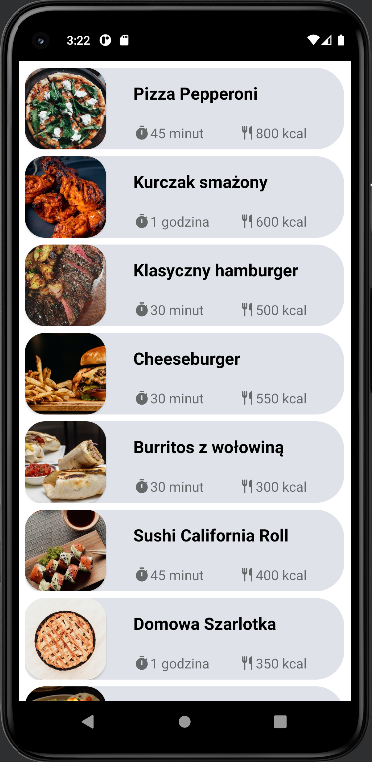
\includegraphics[width=0.4\textwidth]{"imgs/phone_list.png"} \\
              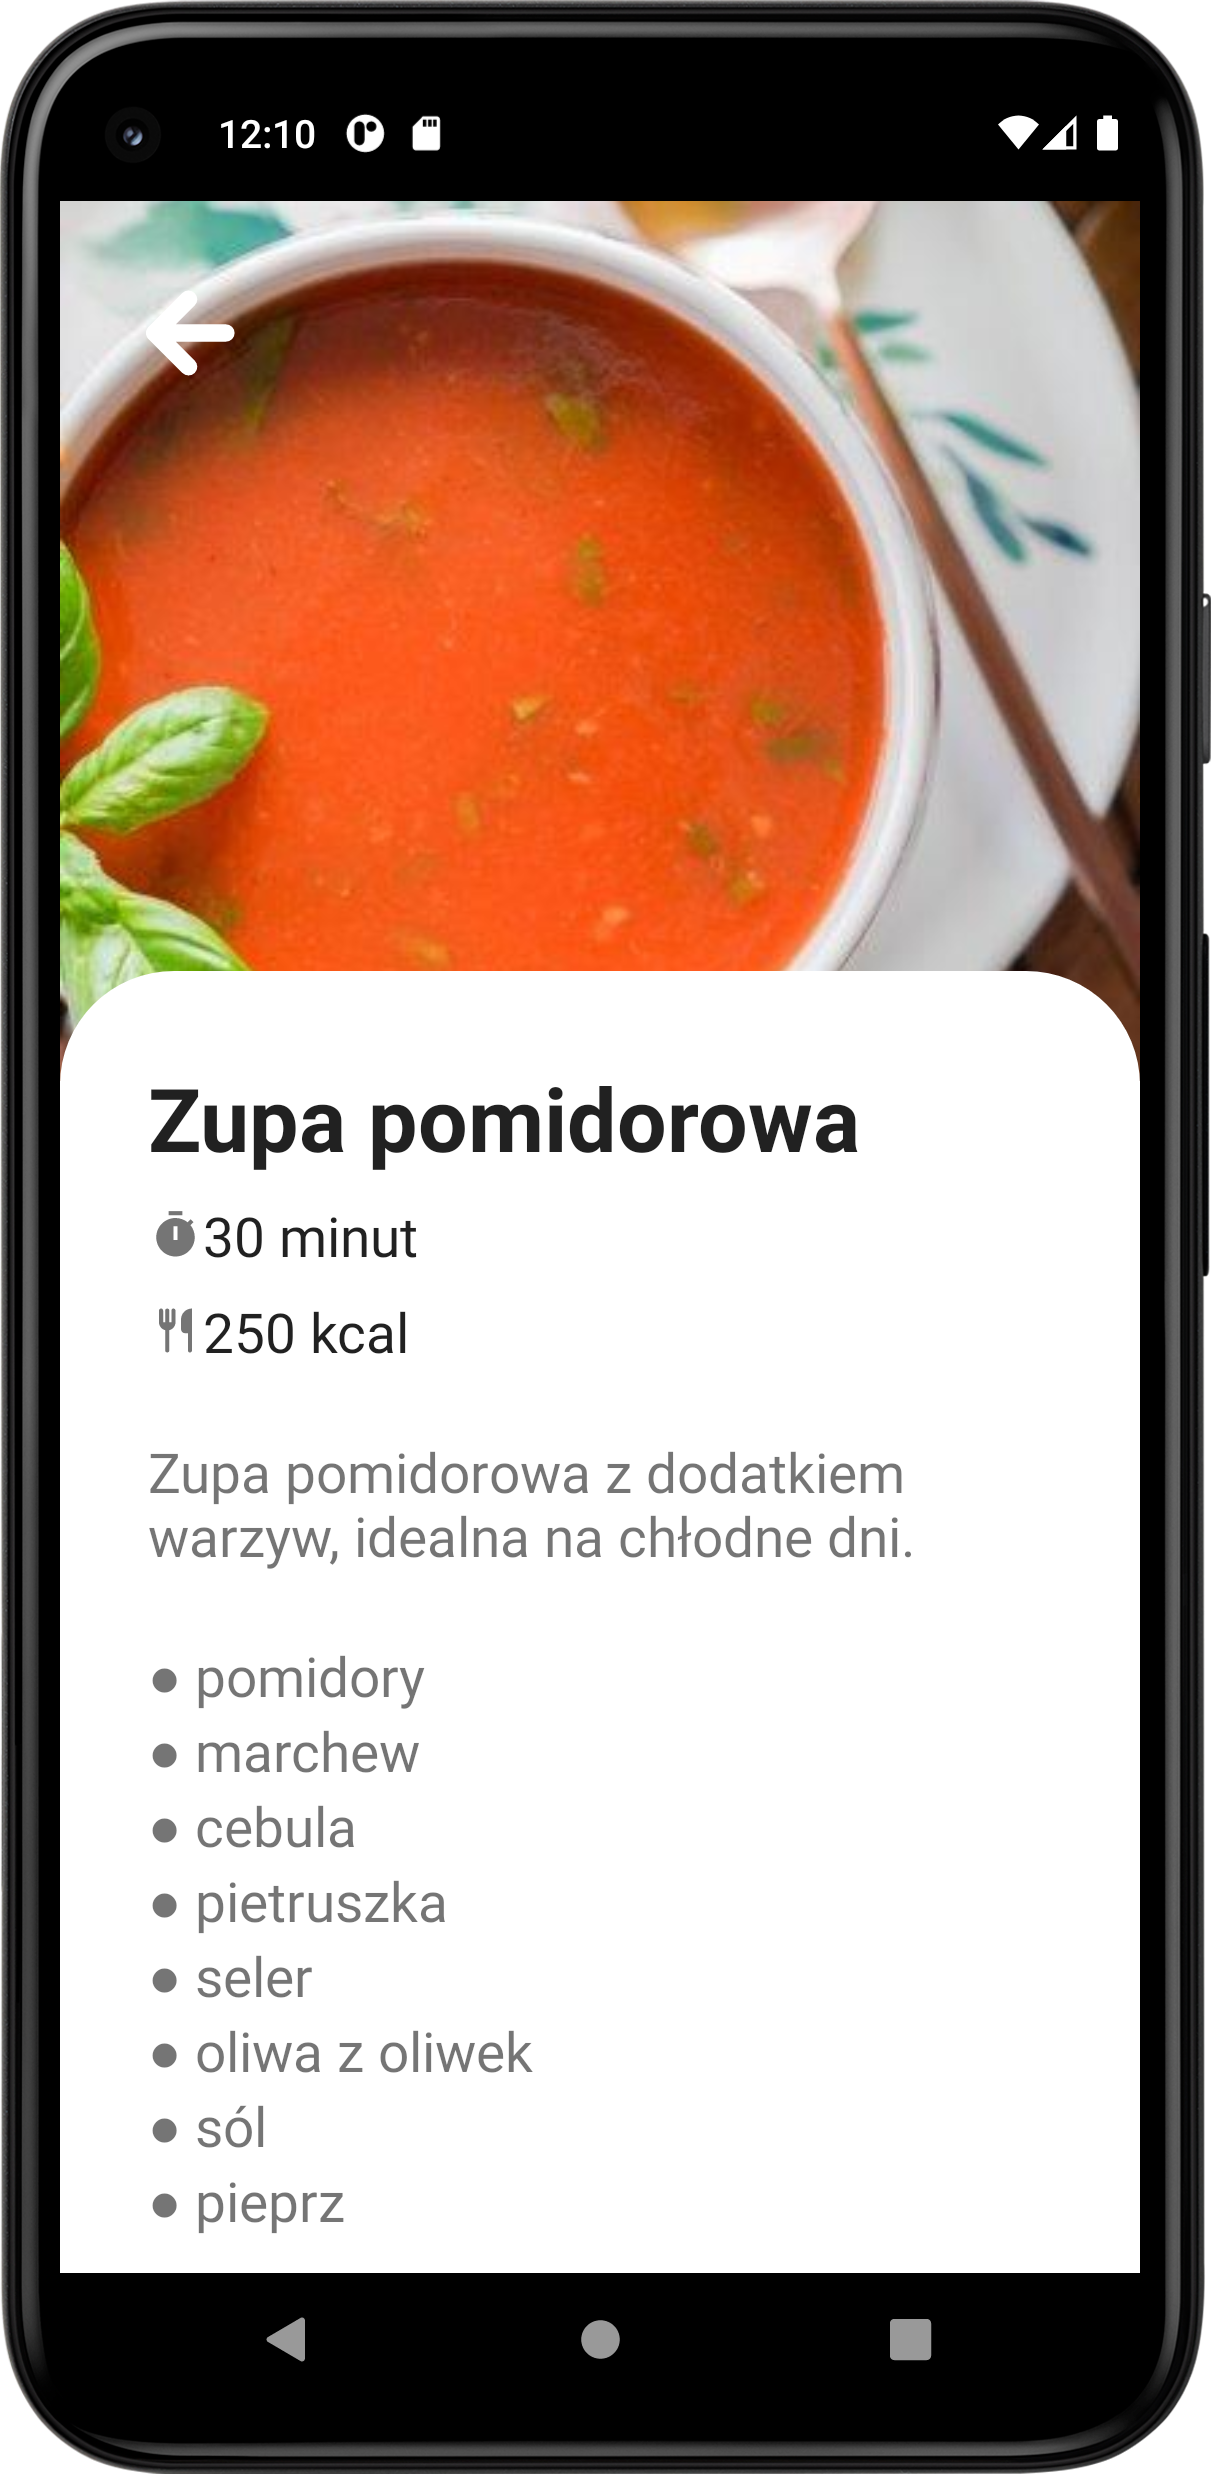
\includegraphics[width=0.4\textwidth]{"imgs/phone_recipe_detail.png"} \\
              \item Implementacja dwóch wersji układu: dla smartfonów oraz dla tabletów.
              \item Implementacja obsługi zmiany orientacji urządzenia
              \item Wykorzystanie fragmentów
              \item W celu uzyskania informacji o przepisach aplikacja korzysta z 
              \item Kod aplikacji jest napisany w Kotlinie
              \item W aplikacji dodane zostały informacje o kaloryczności potrawy
          \end{enumerate}
\end{enumerate}
\end{document}
